\documentclass[a4paper]{book}
\usepackage{makeidx}
\usepackage{natbib}
\usepackage{graphicx}
\usepackage{multicol}
\usepackage{float}
\usepackage{listings}
\usepackage{color}
\usepackage{ifthen}
\usepackage[table]{xcolor}
\usepackage{textcomp}
\usepackage{alltt}
\usepackage{ifpdf}
\ifpdf
\usepackage[pdftex,
            pagebackref=true,
            colorlinks=true,
            linkcolor=blue,
            unicode
           ]{hyperref}
\else
\usepackage[ps2pdf,
            pagebackref=true,
            colorlinks=true,
            linkcolor=blue,
            unicode
           ]{hyperref}
\usepackage{pspicture}
\fi
\usepackage[utf8]{inputenc}
\usepackage{mathptmx}
\usepackage[scaled=.90]{helvet}
\usepackage{courier}
\usepackage{sectsty}
\usepackage[titles]{tocloft}
\usepackage{doxygen}
\lstset{language=C++,inputencoding=utf8,basicstyle=\footnotesize,breaklines=true,breakatwhitespace=true,tabsize=8,numbers=left }
\makeindex
\setcounter{tocdepth}{3}
\renewcommand{\footrulewidth}{0.4pt}
\renewcommand{\familydefault}{\sfdefault}
\hfuzz=15pt
\setlength{\emergencystretch}{15pt}
\hbadness=750
\tolerance=750
\begin{document}
\hypersetup{pageanchor=false,citecolor=blue}
\begin{titlepage}
\vspace*{7cm}
\begin{center}
{\Large \-Club\-Engine \-P\-L\-T \\[1ex]\large 1 }\\
\vspace*{1cm}
{\large \-Generated by Doxygen 1.7.6.1}\\
\vspace*{0.5cm}
{\small Fri Jan 24 2014 23:39:00}\\
\end{center}
\end{titlepage}
\clearemptydoublepage
\pagenumbering{roman}
\tableofcontents
\clearemptydoublepage
\pagenumbering{arabic}
\hypersetup{pageanchor=true,citecolor=blue}
\chapter{\-Class \-Index}
\section{\-Class \-Hierarchy}
\-This inheritance list is sorted roughly, but not completely, alphabetically\-:\begin{DoxyCompactList}
\item \contentsline{section}{\-Abstract\-State\-Factory}{\pageref{classAbstractStateFactory}}{}
\begin{DoxyCompactList}
\item \contentsline{section}{\-My\-State\-Factory}{\pageref{classMyStateFactory}}{}
\end{DoxyCompactList}
\item \contentsline{section}{\-Application}{\pageref{classApplication}}{}
\item \contentsline{section}{\-Context}{\pageref{classContext}}{}
\item \contentsline{section}{\-Map}{\pageref{classMap}}{}
\item \contentsline{section}{\-State\-Stack\-:\-:\-Pending\-Change}{\pageref{structStateStack_1_1PendingChange}}{}
\item \contentsline{section}{\-Game\-State\-:\-:selected}{\pageref{structGameState_1_1selected}}{}
\item \contentsline{section}{\-Sound\-Holder}{\pageref{classSoundHolder}}{}
\item \contentsline{section}{\-State}{\pageref{classState}}{}
\begin{DoxyCompactList}
\item \contentsline{section}{\-Debug\-State}{\pageref{classDebugState}}{}
\item \contentsline{section}{\-Game\-State}{\pageref{classGameState}}{}
\item \contentsline{section}{\-Pause\-State}{\pageref{classPauseState}}{}
\item \contentsline{section}{\-Test\-State}{\pageref{classTestState}}{}
\item \contentsline{section}{\-Title\-State}{\pageref{classTitleState}}{}
\end{DoxyCompactList}
\item \contentsline{section}{\-State\-Stack}{\pageref{classStateStack}}{}
\item \contentsline{section}{\-Texture\-Holder}{\pageref{classTextureHolder}}{}
\end{DoxyCompactList}

\chapter{\-Class \-Index}
\section{\-Class \-List}
\-Here are the classes, structs, unions and interfaces with brief descriptions\-:\begin{DoxyCompactList}
\item\contentsline{section}{\hyperlink{classAbstractStateFactory}{\-Abstract\-State\-Factory} }{\pageref{classAbstractStateFactory}}{}
\item\contentsline{section}{\hyperlink{classApplication}{\-Application} }{\pageref{classApplication}}{}
\item\contentsline{section}{\hyperlink{classContext}{\-Context} }{\pageref{classContext}}{}
\item\contentsline{section}{\hyperlink{classDebugState}{\-Debug\-State} }{\pageref{classDebugState}}{}
\item\contentsline{section}{\hyperlink{classGameState}{\-Game\-State} }{\pageref{classGameState}}{}
\item\contentsline{section}{\hyperlink{classMap}{\-Map} }{\pageref{classMap}}{}
\item\contentsline{section}{\hyperlink{classMyStateFactory}{\-My\-State\-Factory} }{\pageref{classMyStateFactory}}{}
\item\contentsline{section}{\hyperlink{classPauseState}{\-Pause\-State} }{\pageref{classPauseState}}{}
\item\contentsline{section}{\hyperlink{structStateStack_1_1PendingChange}{\-State\-Stack\-::\-Pending\-Change} }{\pageref{structStateStack_1_1PendingChange}}{}
\item\contentsline{section}{\hyperlink{structGameState_1_1selected}{\-Game\-State\-::selected} }{\pageref{structGameState_1_1selected}}{}
\item\contentsline{section}{\hyperlink{classSoundHolder}{\-Sound\-Holder} }{\pageref{classSoundHolder}}{}
\item\contentsline{section}{\hyperlink{classState}{\-State} }{\pageref{classState}}{}
\item\contentsline{section}{\hyperlink{classStateStack}{\-State\-Stack} }{\pageref{classStateStack}}{}
\item\contentsline{section}{\hyperlink{classTestState}{\-Test\-State} }{\pageref{classTestState}}{}
\item\contentsline{section}{\hyperlink{classTextureHolder}{\-Texture\-Holder} }{\pageref{classTextureHolder}}{}
\item\contentsline{section}{\hyperlink{classTitleState}{\-Title\-State} }{\pageref{classTitleState}}{}
\end{DoxyCompactList}

\chapter{\-Class \-Documentation}
\hypertarget{classAbstractStateFactory}{\section{\-Abstract\-State\-Factory \-Class \-Reference}
\label{classAbstractStateFactory}\index{\-Abstract\-State\-Factory@{\-Abstract\-State\-Factory}}
}
\-Inheritance diagram for \-Abstract\-State\-Factory\-:\begin{figure}[H]
\begin{center}
\leavevmode
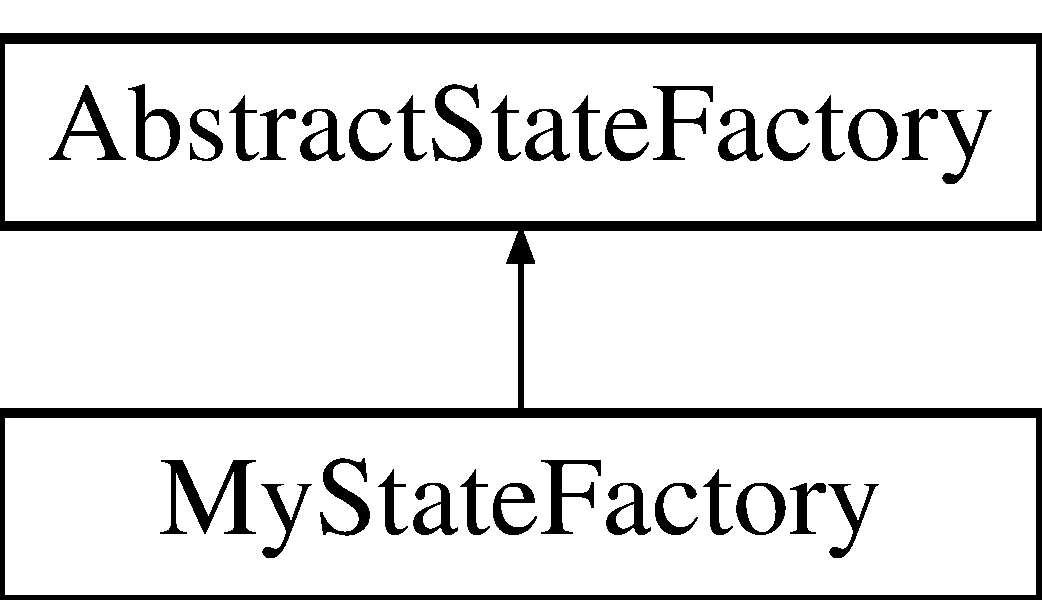
\includegraphics[height=2.000000cm]{classAbstractStateFactory}
\end{center}
\end{figure}
\subsection*{\-Public \-Member \-Functions}
\begin{DoxyCompactItemize}
\item 
\hypertarget{classAbstractStateFactory_aa009b802527e422ca064d8f4cae95a90_aa009b802527e422ca064d8f4cae95a90}{virtual \hyperlink{classState}{\-State} $\ast$ {\bfseries get} (\-States\-::\-I\-D id, \hyperlink{classStateStack}{\-State\-Stack} \&state\-Stack, \hyperlink{classContext}{\-Context} \&context)=0}\label{classAbstractStateFactory_aa009b802527e422ca064d8f4cae95a90_aa009b802527e422ca064d8f4cae95a90}

\end{DoxyCompactItemize}


\-The documentation for this class was generated from the following files\-:\begin{DoxyCompactItemize}
\item 
core/state/\-Abstract\-State\-Factory.\-hpp\item 
core/state/\-Abstract\-State\-Factory.\-cpp\end{DoxyCompactItemize}

\hypertarget{classApplication}{\section{\-Application \-Class \-Reference}
\label{classApplication}\index{\-Application@{\-Application}}
}
\subsection*{\-Public \-Member \-Functions}
\begin{DoxyCompactItemize}
\item 
\hypertarget{classApplication_a328ef40e03ee2fe1d68dd34e2be5e80c_a328ef40e03ee2fe1d68dd34e2be5e80c}{{\bfseries \-Application} (\hyperlink{classAbstractStateFactory}{\-Abstract\-State\-Factory} \&factory)}\label{classApplication_a328ef40e03ee2fe1d68dd34e2be5e80c_a328ef40e03ee2fe1d68dd34e2be5e80c}

\item 
\hypertarget{classApplication_a68965449404743bf1add056784d6cf81_a68965449404743bf1add056784d6cf81}{void {\bfseries run} ()}\label{classApplication_a68965449404743bf1add056784d6cf81_a68965449404743bf1add056784d6cf81}

\item 
\hypertarget{classApplication_a0603f060b53ea465da8a80d625429d10_a0603f060b53ea465da8a80d625429d10}{void {\bfseries push\-State} (\-States\-::\-I\-D id)}\label{classApplication_a0603f060b53ea465da8a80d625429d10_a0603f060b53ea465da8a80d625429d10}

\end{DoxyCompactItemize}
\subsection*{\-Private \-Member \-Functions}
\begin{DoxyCompactItemize}
\item 
\hypertarget{classApplication_a157472e00e1db5fced576a262c866702_a157472e00e1db5fced576a262c866702}{void {\bfseries process\-Inputs} ()}\label{classApplication_a157472e00e1db5fced576a262c866702_a157472e00e1db5fced576a262c866702}

\item 
\hypertarget{classApplication_aa1493bab632d6909708b0dc214f464de_aa1493bab632d6909708b0dc214f464de}{void {\bfseries update} (sf\-::\-Time dt)}\label{classApplication_aa1493bab632d6909708b0dc214f464de_aa1493bab632d6909708b0dc214f464de}

\item 
\hypertarget{classApplication_a9ac99d97ee1cc814298a2f2388bde835_a9ac99d97ee1cc814298a2f2388bde835}{void {\bfseries render} ()}\label{classApplication_a9ac99d97ee1cc814298a2f2388bde835_a9ac99d97ee1cc814298a2f2388bde835}

\end{DoxyCompactItemize}
\subsection*{\-Private \-Attributes}
\begin{DoxyCompactItemize}
\item 
\hypertarget{classApplication_ac3e5164a1ec3d2dfaecc6724692d10c3_ac3e5164a1ec3d2dfaecc6724692d10c3}{sf\-::\-Context {\bfseries m\-G\-L\-Context}}\label{classApplication_ac3e5164a1ec3d2dfaecc6724692d10c3_ac3e5164a1ec3d2dfaecc6724692d10c3}

\item 
\hypertarget{classApplication_a1c1480e1f6bd4e2d3fe9a5d2171a5a54_a1c1480e1f6bd4e2d3fe9a5d2171a5a54}{sf\-::\-Render\-Window {\bfseries m\-Window}}\label{classApplication_a1c1480e1f6bd4e2d3fe9a5d2171a5a54_a1c1480e1f6bd4e2d3fe9a5d2171a5a54}

\item 
\hypertarget{classApplication_a5b885fafceb746e25b88a7afecf1e811_a5b885fafceb746e25b88a7afecf1e811}{\hyperlink{classTextureHolder}{\-Texture\-Holder} {\bfseries m\-Texture\-Holder}}\label{classApplication_a5b885fafceb746e25b88a7afecf1e811_a5b885fafceb746e25b88a7afecf1e811}

\item 
\hypertarget{classApplication_a0a84a8c5be50884234d0499833b82c26_a0a84a8c5be50884234d0499833b82c26}{\hyperlink{classSoundHolder}{\-Sound\-Holder} {\bfseries m\-Sound\-Holder}}\label{classApplication_a0a84a8c5be50884234d0499833b82c26_a0a84a8c5be50884234d0499833b82c26}

\item 
\hypertarget{classApplication_a8b01542499e71a40c2ed277cac4b6abe_a8b01542499e71a40c2ed277cac4b6abe}{\hyperlink{classStateStack}{\-State\-Stack} {\bfseries m\-State\-Stack}}\label{classApplication_a8b01542499e71a40c2ed277cac4b6abe_a8b01542499e71a40c2ed277cac4b6abe}

\end{DoxyCompactItemize}
\subsection*{\-Static \-Private \-Attributes}
\begin{DoxyCompactItemize}
\item 
\hypertarget{classApplication_a0c54e0e34ffc2c1354902604a7038b37_a0c54e0e34ffc2c1354902604a7038b37}{static const sf\-::\-Time {\bfseries \-Time\-Per\-Frame} = sf\-::seconds(1.f/60.f)}\label{classApplication_a0c54e0e34ffc2c1354902604a7038b37_a0c54e0e34ffc2c1354902604a7038b37}

\end{DoxyCompactItemize}


\-The documentation for this class was generated from the following files\-:\begin{DoxyCompactItemize}
\item 
core/\-Application.\-hpp\item 
core/\-Application.\-cpp\end{DoxyCompactItemize}

\hypertarget{classContext}{\section{\-Context \-Class \-Reference}
\label{classContext}\index{\-Context@{\-Context}}
}


{\ttfamily \#include $<$\-Context.\-hpp$>$}

\subsection*{\-Public \-Member \-Functions}
\begin{DoxyCompactItemize}
\item 
\hypertarget{classContext_a427f26b033dd1da604f4a63356d332a2_a427f26b033dd1da604f4a63356d332a2}{{\bfseries \-Context} (sf\-::\-Render\-Window \&\-\_\-window, \hyperlink{classTextureHolder}{\-Texture\-Holder} \&\-\_\-textures, \hyperlink{classSoundHolder}{\-Sound\-Holder} \&\-\_\-sounds)}\label{classContext_a427f26b033dd1da604f4a63356d332a2_a427f26b033dd1da604f4a63356d332a2}

\end{DoxyCompactItemize}
\subsection*{\-Public \-Attributes}
\begin{DoxyCompactItemize}
\item 
\hypertarget{classContext_adfd0cc74ffbdf3f22ae41f4114afb296_adfd0cc74ffbdf3f22ae41f4114afb296}{sf\-::\-Render\-Window $\ast$ {\bfseries window}}\label{classContext_adfd0cc74ffbdf3f22ae41f4114afb296_adfd0cc74ffbdf3f22ae41f4114afb296}

\item 
\hypertarget{classContext_a17045faaf6066a6430c6cf97151b29df_a17045faaf6066a6430c6cf97151b29df}{\hyperlink{classTextureHolder}{\-Texture\-Holder} $\ast$ {\bfseries textures}}\label{classContext_a17045faaf6066a6430c6cf97151b29df_a17045faaf6066a6430c6cf97151b29df}

\item 
\hypertarget{classContext_a864a15210fffe920e5bddf95fd135456_a864a15210fffe920e5bddf95fd135456}{\hyperlink{classSoundHolder}{\-Sound\-Holder} $\ast$ {\bfseries sounds}}\label{classContext_a864a15210fffe920e5bddf95fd135456_a864a15210fffe920e5bddf95fd135456}

\end{DoxyCompactItemize}


\subsection{\-Detailed \-Description}
\-Contain global resources for states 

\-The documentation for this class was generated from the following file\-:\begin{DoxyCompactItemize}
\item 
core/\-Context.\-hpp\end{DoxyCompactItemize}

\hypertarget{classDebugState}{\section{\-Debug\-State \-Class \-Reference}
\label{classDebugState}\index{\-Debug\-State@{\-Debug\-State}}
}
\-Inheritance diagram for \-Debug\-State\-:\begin{figure}[H]
\begin{center}
\leavevmode
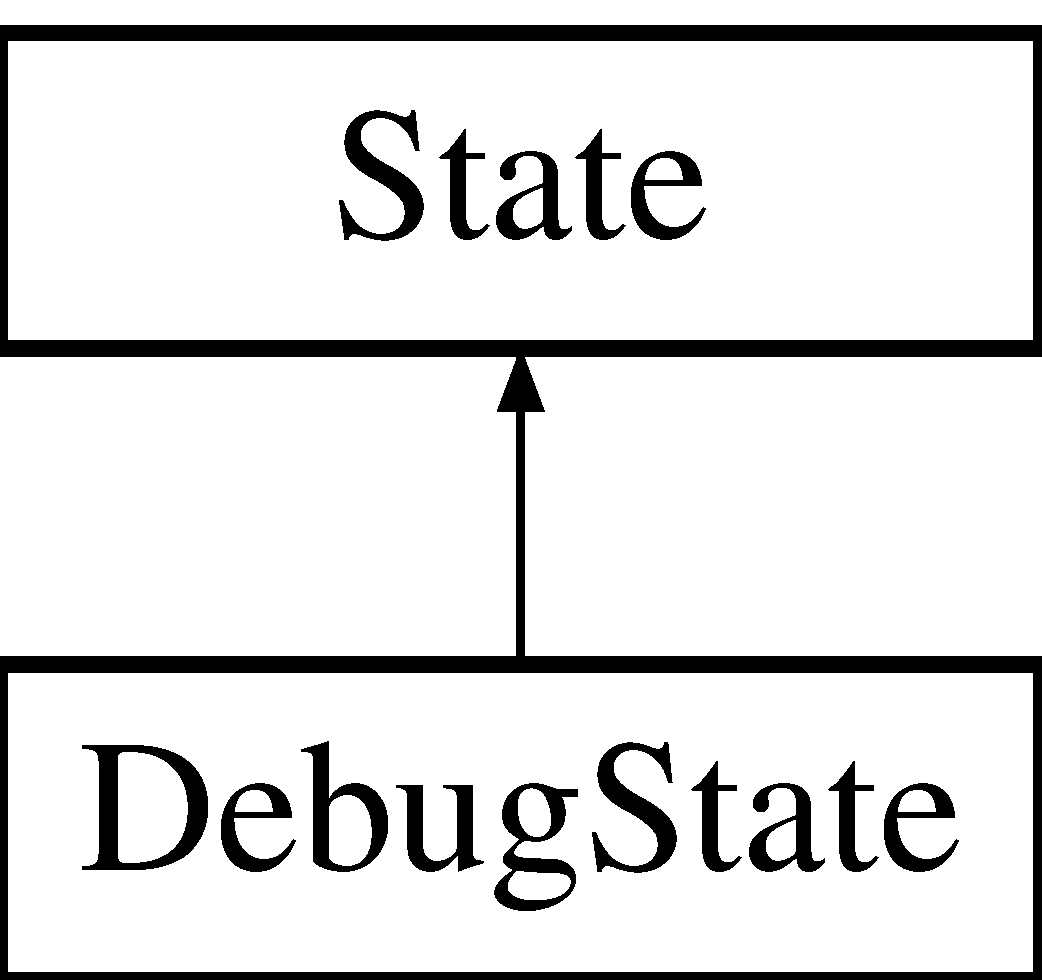
\includegraphics[height=2.000000cm]{classDebugState}
\end{center}
\end{figure}
\subsection*{\-Public \-Member \-Functions}
\begin{DoxyCompactItemize}
\item 
\hypertarget{classDebugState_aa8678f0606f489204d04c130c9a2b073_aa8678f0606f489204d04c130c9a2b073}{{\bfseries \-Debug\-State} (\hyperlink{classStateStack}{\-State\-Stack} \&stack, \hyperlink{classContext}{\-Context} \&context)}\label{classDebugState_aa8678f0606f489204d04c130c9a2b073_aa8678f0606f489204d04c130c9a2b073}

\item 
virtual bool \hyperlink{classDebugState_aef82c5d07e51ab4ea7abcade50370ae2_aef82c5d07e51ab4ea7abcade50370ae2}{handle\-Event} (const sf\-::\-Event \&event)
\item 
virtual bool \hyperlink{classDebugState_a6f49614c9b947cedcad131c28e24f885_a6f49614c9b947cedcad131c28e24f885}{update} (sf\-::\-Time dt)
\item 
\hypertarget{classDebugState_a716ecec331e20d4efa31b9de46381669_a716ecec331e20d4efa31b9de46381669}{virtual void {\bfseries draw} ()}\label{classDebugState_a716ecec331e20d4efa31b9de46381669_a716ecec331e20d4efa31b9de46381669}

\end{DoxyCompactItemize}


\subsection{\-Member \-Function \-Documentation}
\hypertarget{classDebugState_aef82c5d07e51ab4ea7abcade50370ae2_aef82c5d07e51ab4ea7abcade50370ae2}{\index{\-Debug\-State@{\-Debug\-State}!handle\-Event@{handle\-Event}}
\index{handle\-Event@{handle\-Event}!DebugState@{\-Debug\-State}}
\subsubsection[{handle\-Event}]{\setlength{\rightskip}{0pt plus 5cm}bool {\bf \-Debug\-State\-::handle\-Event} (
\begin{DoxyParamCaption}
\item[{const sf\-::\-Event \&}]{event}
\end{DoxyParamCaption}
)\hspace{0.3cm}{\ttfamily  \mbox{[}virtual\mbox{]}}}}\label{classDebugState_aef82c5d07e51ab4ea7abcade50370ae2_aef82c5d07e51ab4ea7abcade50370ae2}
\-Return false to stop states updating 

\-Implements \hyperlink{classState_a19965f83460b248c42952aac8d001206_a19965f83460b248c42952aac8d001206}{\-State}.

\hypertarget{classDebugState_a6f49614c9b947cedcad131c28e24f885_a6f49614c9b947cedcad131c28e24f885}{\index{\-Debug\-State@{\-Debug\-State}!update@{update}}
\index{update@{update}!DebugState@{\-Debug\-State}}
\subsubsection[{update}]{\setlength{\rightskip}{0pt plus 5cm}bool {\bf \-Debug\-State\-::update} (
\begin{DoxyParamCaption}
\item[{sf\-::\-Time}]{dt}
\end{DoxyParamCaption}
)\hspace{0.3cm}{\ttfamily  \mbox{[}virtual\mbox{]}}}}\label{classDebugState_a6f49614c9b947cedcad131c28e24f885_a6f49614c9b947cedcad131c28e24f885}
\-Return false to stop states updating 

\-Implements \hyperlink{classState_acd5926bc7a373edff9e57f3ffe94ca13_acd5926bc7a373edff9e57f3ffe94ca13}{\-State}.



\-The documentation for this class was generated from the following files\-:\begin{DoxyCompactItemize}
\item 
core/state/\-Debug\-State.\-hpp\item 
core/state/\-Debug\-State.\-cpp\end{DoxyCompactItemize}

\hypertarget{classGameState}{\section{\-Game\-State \-Class \-Reference}
\label{classGameState}\index{\-Game\-State@{\-Game\-State}}
}
\-Inheritance diagram for \-Game\-State\-:\begin{figure}[H]
\begin{center}
\leavevmode
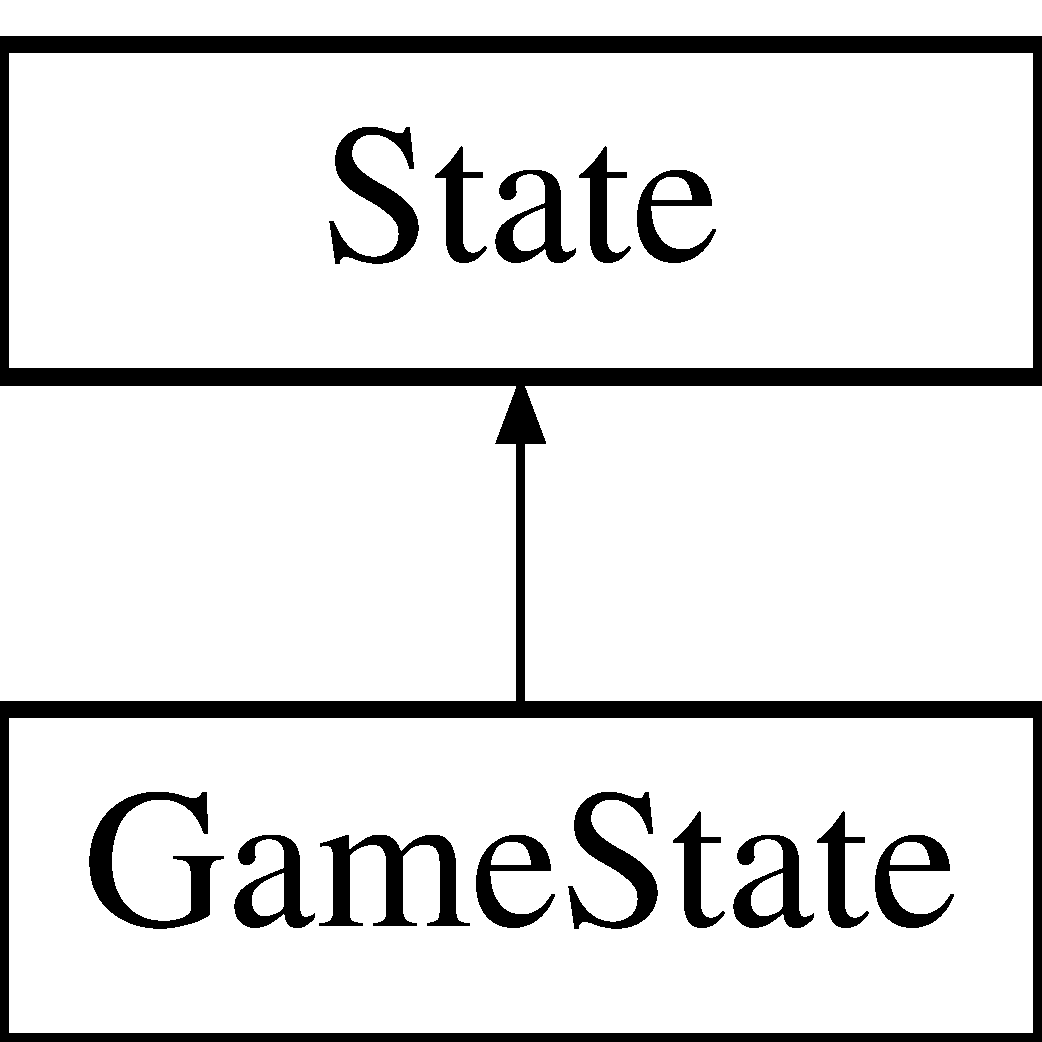
\includegraphics[height=2.000000cm]{classGameState}
\end{center}
\end{figure}
\subsection*{\-Classes}
\begin{DoxyCompactItemize}
\item 
struct \hyperlink{structGameState_1_1selected}{selected}
\end{DoxyCompactItemize}
\subsection*{\-Public \-Member \-Functions}
\begin{DoxyCompactItemize}
\item 
\hypertarget{classGameState_aa7d21e6d14f32ba7c2e155a9905b81aa_aa7d21e6d14f32ba7c2e155a9905b81aa}{{\bfseries \-Game\-State} (\hyperlink{classStateStack}{\-State\-Stack} \&stack, \hyperlink{classContext}{\-Context} \&context)}\label{classGameState_aa7d21e6d14f32ba7c2e155a9905b81aa_aa7d21e6d14f32ba7c2e155a9905b81aa}

\item 
virtual bool \hyperlink{classGameState_a000dd3306b1cb9faab5a86774a22aa6d_a000dd3306b1cb9faab5a86774a22aa6d}{handle\-Event} (const sf\-::\-Event \&event)
\item 
virtual bool \hyperlink{classGameState_a4ac988f0da5c33b43ff356890fcf9c1c_a4ac988f0da5c33b43ff356890fcf9c1c}{update} (sf\-::\-Time dt)
\item 
\hypertarget{classGameState_a3c511417d8934943ae65c04681f321a3_a3c511417d8934943ae65c04681f321a3}{virtual void {\bfseries draw} ()}\label{classGameState_a3c511417d8934943ae65c04681f321a3_a3c511417d8934943ae65c04681f321a3}

\end{DoxyCompactItemize}
\subsection*{\-Private \-Attributes}
\begin{DoxyCompactItemize}
\item 
\hypertarget{classGameState_a63a1d1e3f644331ed1d38fac12f0de82_a63a1d1e3f644331ed1d38fac12f0de82}{int {\bfseries lol}}\label{classGameState_a63a1d1e3f644331ed1d38fac12f0de82_a63a1d1e3f644331ed1d38fac12f0de82}

\item 
\hypertarget{classGameState_a5461ce079b93c1a1fb52199af6b21629_a5461ce079b93c1a1fb52199af6b21629}{bool {\bfseries mouseispressed}}\label{classGameState_a5461ce079b93c1a1fb52199af6b21629_a5461ce079b93c1a1fb52199af6b21629}

\item 
\hypertarget{classGameState_a840248426d5f4d682a5a46dbe865c01d_a840248426d5f4d682a5a46dbe865c01d}{float {\bfseries aux}}\label{classGameState_a840248426d5f4d682a5a46dbe865c01d_a840248426d5f4d682a5a46dbe865c01d}

\item 
\hypertarget{classGameState_aa05df59ca1bb66f1ce5524cbc6fcac3d_aa05df59ca1bb66f1ce5524cbc6fcac3d}{\hyperlink{structGameState_1_1selected}{selected} {\bfseries selected}}\label{classGameState_aa05df59ca1bb66f1ce5524cbc6fcac3d_aa05df59ca1bb66f1ce5524cbc6fcac3d}

\item 
\hypertarget{classGameState_a87df533b5aa84d3fe41fbaf1d5ec8861_a87df533b5aa84d3fe41fbaf1d5ec8861}{int {\bfseries width}}\label{classGameState_a87df533b5aa84d3fe41fbaf1d5ec8861_a87df533b5aa84d3fe41fbaf1d5ec8861}

\item 
\hypertarget{classGameState_ad5cc108fdbfdd24fa5d8897b680438bc_ad5cc108fdbfdd24fa5d8897b680438bc}{int {\bfseries height}}\label{classGameState_ad5cc108fdbfdd24fa5d8897b680438bc_ad5cc108fdbfdd24fa5d8897b680438bc}

\item 
\hypertarget{classGameState_ada30b3ee0f083563f7b1d28e8bcf10ce_ada30b3ee0f083563f7b1d28e8bcf10ce}{int {\bfseries tile\-Size}}\label{classGameState_ada30b3ee0f083563f7b1d28e8bcf10ce_ada30b3ee0f083563f7b1d28e8bcf10ce}

\item 
\hypertarget{classGameState_a660ea9817bdd451f5ffffaf18fae63e9_a660ea9817bdd451f5ffffaf18fae63e9}{\hyperlink{classMap}{\-Map} $\ast$ {\bfseries map}}\label{classGameState_a660ea9817bdd451f5ffffaf18fae63e9_a660ea9817bdd451f5ffffaf18fae63e9}

\item 
\hypertarget{classGameState_a9dd8bced38e96ba91a1d95a6c8cbeab4_a9dd8bced38e96ba91a1d95a6c8cbeab4}{sf\-::\-Texture {\bfseries grid}}\label{classGameState_a9dd8bced38e96ba91a1d95a6c8cbeab4_a9dd8bced38e96ba91a1d95a6c8cbeab4}

\item 
\hypertarget{classGameState_a0c86e04c6d92c157785a446140aca6d0_a0c86e04c6d92c157785a446140aca6d0}{sf\-::\-Sprite {\bfseries gridsprite}}\label{classGameState_a0c86e04c6d92c157785a446140aca6d0_a0c86e04c6d92c157785a446140aca6d0}

\item 
\hypertarget{classGameState_a768594ad10d1ac7f832f30f120f2cc57_a768594ad10d1ac7f832f30f120f2cc57}{sf\-::\-Rectangle\-Shape {\bfseries selection}}\label{classGameState_a768594ad10d1ac7f832f30f120f2cc57_a768594ad10d1ac7f832f30f120f2cc57}

\end{DoxyCompactItemize}


\subsection{\-Member \-Function \-Documentation}
\hypertarget{classGameState_a000dd3306b1cb9faab5a86774a22aa6d_a000dd3306b1cb9faab5a86774a22aa6d}{\index{\-Game\-State@{\-Game\-State}!handle\-Event@{handle\-Event}}
\index{handle\-Event@{handle\-Event}!GameState@{\-Game\-State}}
\subsubsection[{handle\-Event}]{\setlength{\rightskip}{0pt plus 5cm}bool {\bf \-Game\-State\-::handle\-Event} (
\begin{DoxyParamCaption}
\item[{const sf\-::\-Event \&}]{event}
\end{DoxyParamCaption}
)\hspace{0.3cm}{\ttfamily  \mbox{[}virtual\mbox{]}}}}\label{classGameState_a000dd3306b1cb9faab5a86774a22aa6d_a000dd3306b1cb9faab5a86774a22aa6d}
\-Return false to stop states updating 

\-Implements \hyperlink{classState_a19965f83460b248c42952aac8d001206_a19965f83460b248c42952aac8d001206}{\-State}.

\hypertarget{classGameState_a4ac988f0da5c33b43ff356890fcf9c1c_a4ac988f0da5c33b43ff356890fcf9c1c}{\index{\-Game\-State@{\-Game\-State}!update@{update}}
\index{update@{update}!GameState@{\-Game\-State}}
\subsubsection[{update}]{\setlength{\rightskip}{0pt plus 5cm}bool {\bf \-Game\-State\-::update} (
\begin{DoxyParamCaption}
\item[{sf\-::\-Time}]{dt}
\end{DoxyParamCaption}
)\hspace{0.3cm}{\ttfamily  \mbox{[}virtual\mbox{]}}}}\label{classGameState_a4ac988f0da5c33b43ff356890fcf9c1c_a4ac988f0da5c33b43ff356890fcf9c1c}
\-Return false to stop states updating 

\-Implements \hyperlink{classState_acd5926bc7a373edff9e57f3ffe94ca13_acd5926bc7a373edff9e57f3ffe94ca13}{\-State}.



\-The documentation for this class was generated from the following files\-:\begin{DoxyCompactItemize}
\item 
gameplay/\-Game\-State.\-hpp\item 
gameplay/\-Game\-State.\-cpp\end{DoxyCompactItemize}

\hypertarget{classMap}{\section{\-Map \-Class \-Reference}
\label{classMap}\index{\-Map@{\-Map}}
}
\subsection*{\-Public \-Member \-Functions}
\begin{DoxyCompactItemize}
\item 
\hypertarget{classMap_a2e5d5887bbcec76bf601b7e531667be1_a2e5d5887bbcec76bf601b7e531667be1}{{\bfseries \-Map} (\hyperlink{classContext}{\-Context} \&context, int nbcols, int nbrows)}\label{classMap_a2e5d5887bbcec76bf601b7e531667be1_a2e5d5887bbcec76bf601b7e531667be1}

\item 
\hypertarget{classMap_ab3c5359d2a854207d0dae015ed1ab8c0_ab3c5359d2a854207d0dae015ed1ab8c0}{int {\bfseries get\-Tile} (int i, int j)}\label{classMap_ab3c5359d2a854207d0dae015ed1ab8c0_ab3c5359d2a854207d0dae015ed1ab8c0}

\item 
\hypertarget{classMap_ad4f7841ff5acdb2bee843a7f77c14254_ad4f7841ff5acdb2bee843a7f77c14254}{void {\bfseries set\-Tile} (int i, int j, int state)}\label{classMap_ad4f7841ff5acdb2bee843a7f77c14254_ad4f7841ff5acdb2bee843a7f77c14254}

\item 
\hypertarget{classMap_a9770d585264af2132c92fc6aad6af755_a9770d585264af2132c92fc6aad6af755}{void {\bfseries \-Display} (sf\-::\-Render\-Window $\ast$render\-\_\-win)}\label{classMap_a9770d585264af2132c92fc6aad6af755_a9770d585264af2132c92fc6aad6af755}

\end{DoxyCompactItemize}
\subsection*{\-Private \-Member \-Functions}
\begin{DoxyCompactItemize}
\item 
\hypertarget{classMap_a360398252d37c9fbb1143d2ab156b9f6_a360398252d37c9fbb1143d2ab156b9f6}{void {\bfseries \-Display\-Tile} (sf\-::\-Render\-Window $\ast$render\-\_\-win, int i, int j, sf\-::\-Sprite sp)}\label{classMap_a360398252d37c9fbb1143d2ab156b9f6_a360398252d37c9fbb1143d2ab156b9f6}

\end{DoxyCompactItemize}
\subsection*{\-Private \-Attributes}
\begin{DoxyCompactItemize}
\item 
\hypertarget{classMap_a4c29b9198025062730c467e266a8c218_a4c29b9198025062730c467e266a8c218}{int $\ast$ {\bfseries matrix}}\label{classMap_a4c29b9198025062730c467e266a8c218_a4c29b9198025062730c467e266a8c218}

\item 
\hypertarget{classMap_ac4ac0094dcb7bf690f5926398598da2b_ac4ac0094dcb7bf690f5926398598da2b}{int {\bfseries nbrows}}\label{classMap_ac4ac0094dcb7bf690f5926398598da2b_ac4ac0094dcb7bf690f5926398598da2b}

\item 
\hypertarget{classMap_a559091d12056d5b69ac8b6fd34daf25b_a559091d12056d5b69ac8b6fd34daf25b}{int {\bfseries nbcols}}\label{classMap_a559091d12056d5b69ac8b6fd34daf25b_a559091d12056d5b69ac8b6fd34daf25b}

\item 
\hypertarget{classMap_aa8f01ed967a3229ea3f4e88c70f72cf5_aa8f01ed967a3229ea3f4e88c70f72cf5}{int {\bfseries tile\-\_\-size}}\label{classMap_aa8f01ed967a3229ea3f4e88c70f72cf5_aa8f01ed967a3229ea3f4e88c70f72cf5}

\item 
\hypertarget{classMap_a7f224151b91dc91347c94940d184e796_a7f224151b91dc91347c94940d184e796}{sf\-::\-Sprite {\bfseries sprite\-Herbe}}\label{classMap_a7f224151b91dc91347c94940d184e796_a7f224151b91dc91347c94940d184e796}

\item 
\hypertarget{classMap_a37b10dab448586f3e63ccb40423e4592_a37b10dab448586f3e63ccb40423e4592}{sf\-::\-Sprite {\bfseries sprite\-Terre}}\label{classMap_a37b10dab448586f3e63ccb40423e4592_a37b10dab448586f3e63ccb40423e4592}

\item 
\hypertarget{classMap_a752dda66c66d35cb47f135cfd7ac1518_a752dda66c66d35cb47f135cfd7ac1518}{sf\-::\-Sprite {\bfseries sprite\-Stone}}\label{classMap_a752dda66c66d35cb47f135cfd7ac1518_a752dda66c66d35cb47f135cfd7ac1518}

\end{DoxyCompactItemize}


\-The documentation for this class was generated from the following files\-:\begin{DoxyCompactItemize}
\item 
core/map.\-hpp\item 
core/map.\-cpp\end{DoxyCompactItemize}

\hypertarget{classMyStateFactory}{\section{\-My\-State\-Factory \-Class \-Reference}
\label{classMyStateFactory}\index{\-My\-State\-Factory@{\-My\-State\-Factory}}
}
\-Inheritance diagram for \-My\-State\-Factory\-:\begin{figure}[H]
\begin{center}
\leavevmode
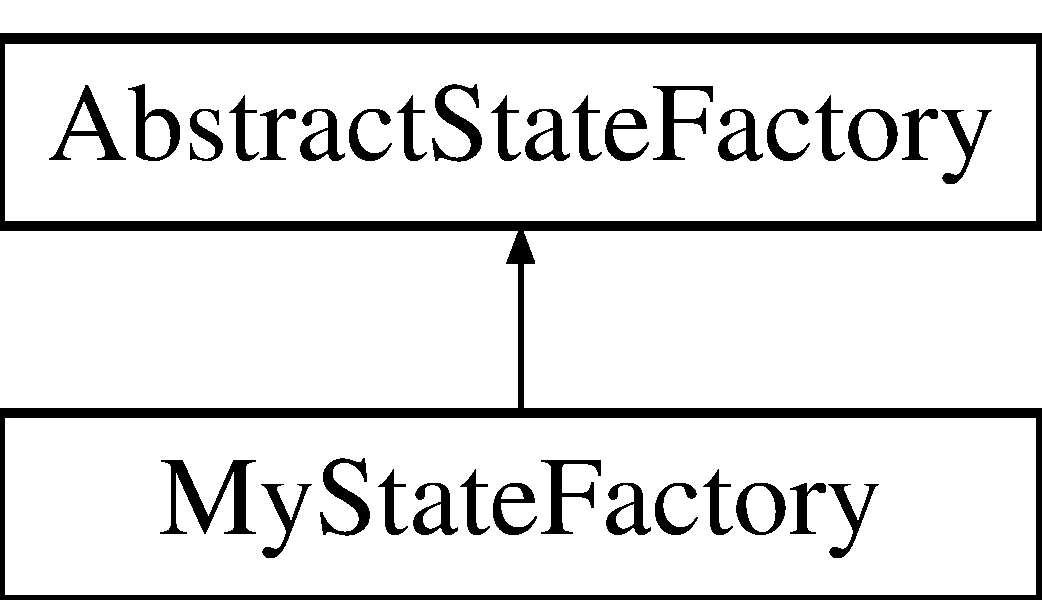
\includegraphics[height=2.000000cm]{classMyStateFactory}
\end{center}
\end{figure}
\subsection*{\-Public \-Member \-Functions}
\begin{DoxyCompactItemize}
\item 
\hypertarget{classMyStateFactory_a2e8344ad4c8aa6ffb65c359dbb034cd7_a2e8344ad4c8aa6ffb65c359dbb034cd7}{virtual \hyperlink{classState}{\-State} $\ast$ {\bfseries get} (\-States\-::\-I\-D id, \hyperlink{classStateStack}{\-State\-Stack} \&state\-Stack, \hyperlink{classContext}{\-Context} \&context)}\label{classMyStateFactory_a2e8344ad4c8aa6ffb65c359dbb034cd7_a2e8344ad4c8aa6ffb65c359dbb034cd7}

\end{DoxyCompactItemize}


\-The documentation for this class was generated from the following files\-:\begin{DoxyCompactItemize}
\item 
gameplay/\-My\-State\-Factory.\-hpp\item 
gameplay/\-My\-State\-Factory.\-cpp\end{DoxyCompactItemize}

\hypertarget{classPauseState}{\section{\-Pause\-State \-Class \-Reference}
\label{classPauseState}\index{\-Pause\-State@{\-Pause\-State}}
}
\-Inheritance diagram for \-Pause\-State\-:\begin{figure}[H]
\begin{center}
\leavevmode
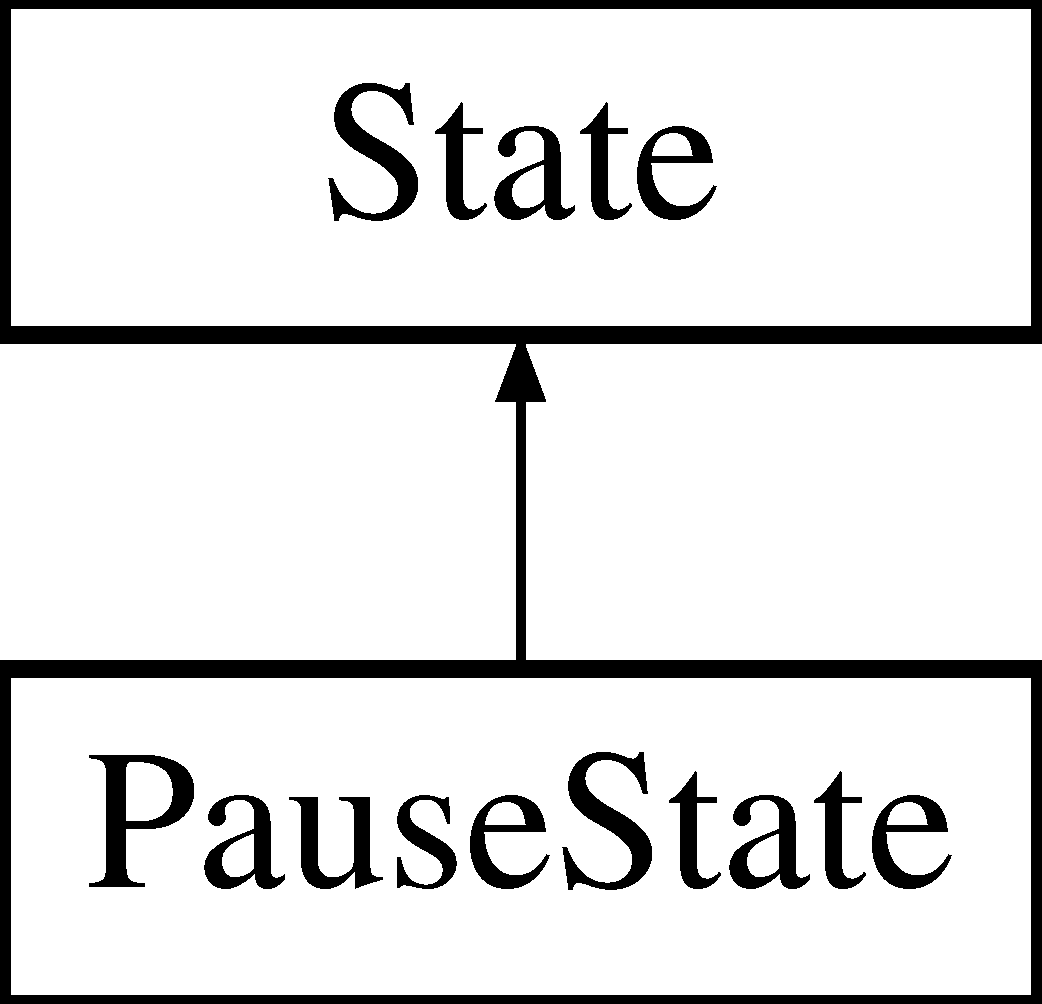
\includegraphics[height=2.000000cm]{classPauseState}
\end{center}
\end{figure}
\subsection*{\-Public \-Member \-Functions}
\begin{DoxyCompactItemize}
\item 
\hypertarget{classPauseState_a09ddb47339507cec238c56de9e1340c2_a09ddb47339507cec238c56de9e1340c2}{{\bfseries \-Pause\-State} (\hyperlink{classStateStack}{\-State\-Stack} \&stack, \hyperlink{classContext}{\-Context} \&context)}\label{classPauseState_a09ddb47339507cec238c56de9e1340c2_a09ddb47339507cec238c56de9e1340c2}

\item 
virtual bool \hyperlink{classPauseState_a685dda66dca3e1c41f4cb02da93c5a8d_a685dda66dca3e1c41f4cb02da93c5a8d}{handle\-Event} (const sf\-::\-Event \&event)
\item 
virtual bool \hyperlink{classPauseState_a9d6e9c6d96e140487badbe1da2738fa3_a9d6e9c6d96e140487badbe1da2738fa3}{update} (sf\-::\-Time dt)
\item 
\hypertarget{classPauseState_ac4c159c2f6d32eedd351f39e36c43f9d_ac4c159c2f6d32eedd351f39e36c43f9d}{virtual void {\bfseries draw} ()}\label{classPauseState_ac4c159c2f6d32eedd351f39e36c43f9d_ac4c159c2f6d32eedd351f39e36c43f9d}

\end{DoxyCompactItemize}


\subsection{\-Member \-Function \-Documentation}
\hypertarget{classPauseState_a685dda66dca3e1c41f4cb02da93c5a8d_a685dda66dca3e1c41f4cb02da93c5a8d}{\index{\-Pause\-State@{\-Pause\-State}!handle\-Event@{handle\-Event}}
\index{handle\-Event@{handle\-Event}!PauseState@{\-Pause\-State}}
\subsubsection[{handle\-Event}]{\setlength{\rightskip}{0pt plus 5cm}bool {\bf \-Pause\-State\-::handle\-Event} (
\begin{DoxyParamCaption}
\item[{const sf\-::\-Event \&}]{event}
\end{DoxyParamCaption}
)\hspace{0.3cm}{\ttfamily  \mbox{[}virtual\mbox{]}}}}\label{classPauseState_a685dda66dca3e1c41f4cb02da93c5a8d_a685dda66dca3e1c41f4cb02da93c5a8d}
\-Return false to stop states updating 

\-Implements \hyperlink{classState_a19965f83460b248c42952aac8d001206_a19965f83460b248c42952aac8d001206}{\-State}.

\hypertarget{classPauseState_a9d6e9c6d96e140487badbe1da2738fa3_a9d6e9c6d96e140487badbe1da2738fa3}{\index{\-Pause\-State@{\-Pause\-State}!update@{update}}
\index{update@{update}!PauseState@{\-Pause\-State}}
\subsubsection[{update}]{\setlength{\rightskip}{0pt plus 5cm}bool {\bf \-Pause\-State\-::update} (
\begin{DoxyParamCaption}
\item[{sf\-::\-Time}]{dt}
\end{DoxyParamCaption}
)\hspace{0.3cm}{\ttfamily  \mbox{[}virtual\mbox{]}}}}\label{classPauseState_a9d6e9c6d96e140487badbe1da2738fa3_a9d6e9c6d96e140487badbe1da2738fa3}
\-Return false to stop states updating 

\-Implements \hyperlink{classState_acd5926bc7a373edff9e57f3ffe94ca13_acd5926bc7a373edff9e57f3ffe94ca13}{\-State}.



\-The documentation for this class was generated from the following files\-:\begin{DoxyCompactItemize}
\item 
gameplay/\-Pause\-State.\-hpp\item 
gameplay/\-Pause\-State.\-cpp\end{DoxyCompactItemize}

\hypertarget{structStateStack_1_1PendingChange}{\section{\-State\-Stack\-:\-:\-Pending\-Change \-Struct \-Reference}
\label{structStateStack_1_1PendingChange}\index{\-State\-Stack\-::\-Pending\-Change@{\-State\-Stack\-::\-Pending\-Change}}
}
\subsection*{\-Public \-Member \-Functions}
\begin{DoxyCompactItemize}
\item 
\hypertarget{structStateStack_1_1PendingChange_adf295f13761e75276203d45bd34d984a_adf295f13761e75276203d45bd34d984a}{{\bfseries \-Pending\-Change} (\-Action action, \-States\-::\-I\-D state\-I\-D=\-States\-::\-None)}\label{structStateStack_1_1PendingChange_adf295f13761e75276203d45bd34d984a_adf295f13761e75276203d45bd34d984a}

\end{DoxyCompactItemize}
\subsection*{\-Public \-Attributes}
\begin{DoxyCompactItemize}
\item 
\hypertarget{structStateStack_1_1PendingChange_a58fbc70279f2e72713293808bbabea08_a58fbc70279f2e72713293808bbabea08}{\-Action {\bfseries action}}\label{structStateStack_1_1PendingChange_a58fbc70279f2e72713293808bbabea08_a58fbc70279f2e72713293808bbabea08}

\item 
\hypertarget{structStateStack_1_1PendingChange_a89163ace43e51d5ce8909e8be1e44c5b_a89163ace43e51d5ce8909e8be1e44c5b}{\-States\-::\-I\-D {\bfseries state\-I\-D}}\label{structStateStack_1_1PendingChange_a89163ace43e51d5ce8909e8be1e44c5b_a89163ace43e51d5ce8909e8be1e44c5b}

\end{DoxyCompactItemize}


\-The documentation for this struct was generated from the following files\-:\begin{DoxyCompactItemize}
\item 
core/state/\-State\-Stack.\-hpp\item 
core/state/\-State\-Stack.\-cpp\end{DoxyCompactItemize}

\hypertarget{structGameState_1_1selected}{\section{\-Game\-State\-:\-:selected \-Struct \-Reference}
\label{structGameState_1_1selected}\index{\-Game\-State\-::selected@{\-Game\-State\-::selected}}
}
\subsection*{\-Public \-Attributes}
\begin{DoxyCompactItemize}
\item 
\hypertarget{structGameState_1_1selected_a60109886e876a63609ba7bd0ed0d6225_a60109886e876a63609ba7bd0ed0d6225}{sf\-::\-Vector2i {\bfseries p1}}\label{structGameState_1_1selected_a60109886e876a63609ba7bd0ed0d6225_a60109886e876a63609ba7bd0ed0d6225}

\item 
\hypertarget{structGameState_1_1selected_a46b1b3f6e16c68379a08d6c2ce3d96b5_a46b1b3f6e16c68379a08d6c2ce3d96b5}{sf\-::\-Vector2i {\bfseries p2}}\label{structGameState_1_1selected_a46b1b3f6e16c68379a08d6c2ce3d96b5_a46b1b3f6e16c68379a08d6c2ce3d96b5}

\item 
\hypertarget{structGameState_1_1selected_a8c0598e1c427893c41a9f06a00b17244_a8c0598e1c427893c41a9f06a00b17244}{sf\-::\-Vector2i {\bfseries i1}}\label{structGameState_1_1selected_a8c0598e1c427893c41a9f06a00b17244_a8c0598e1c427893c41a9f06a00b17244}

\item 
\hypertarget{structGameState_1_1selected_a6fefaa6758e5c0a0fec34ad10ab669d3_a6fefaa6758e5c0a0fec34ad10ab669d3}{sf\-::\-Vector2i {\bfseries i2}}\label{structGameState_1_1selected_a6fefaa6758e5c0a0fec34ad10ab669d3_a6fefaa6758e5c0a0fec34ad10ab669d3}

\end{DoxyCompactItemize}


\-The documentation for this struct was generated from the following file\-:\begin{DoxyCompactItemize}
\item 
gameplay/\-Game\-State.\-hpp\end{DoxyCompactItemize}

\hypertarget{classSoundHolder}{\section{\-Sound\-Holder \-Class \-Reference}
\label{classSoundHolder}\index{\-Sound\-Holder@{\-Sound\-Holder}}
}


{\ttfamily \#include $<$\-Sound\-Holder.\-hpp$>$}

\subsection*{\-Public \-Member \-Functions}
\begin{DoxyCompactItemize}
\item 
\hypertarget{classSoundHolder_aff3a6de65bbfc8b9f5437cfc2a54d91e_aff3a6de65bbfc8b9f5437cfc2a54d91e}{void {\bfseries load} (\-Sounds\-::\-I\-D id, const std\-::string \&filename)}\label{classSoundHolder_aff3a6de65bbfc8b9f5437cfc2a54d91e_aff3a6de65bbfc8b9f5437cfc2a54d91e}

\item 
\hypertarget{classSoundHolder_adfa2c1fc9204dd25189ac1b527de773d_adfa2c1fc9204dd25189ac1b527de773d}{void {\bfseries play} (\-Sounds\-::\-I\-D id)}\label{classSoundHolder_adfa2c1fc9204dd25189ac1b527de773d_adfa2c1fc9204dd25189ac1b527de773d}

\end{DoxyCompactItemize}
\subsection*{\-Private \-Types}
\begin{DoxyCompactItemize}
\item 
\hypertarget{classSoundHolder_a7a84cb257412798b69a722e2d17b35da_a7a84cb257412798b69a722e2d17b35da}{typedef std\-::map$<$ \-Sounds\-::\-I\-D, \*
sf\-::\-Sound\-Buffer $\ast$ $>$ {\bfseries \-Sound\-Map}}\label{classSoundHolder_a7a84cb257412798b69a722e2d17b35da_a7a84cb257412798b69a722e2d17b35da}

\end{DoxyCompactItemize}
\subsection*{\-Private \-Attributes}
\begin{DoxyCompactItemize}
\item 
\hypertarget{classSoundHolder_a58d076b62daad66a7d87184633852df9_a58d076b62daad66a7d87184633852df9}{\-Sound\-Map {\bfseries m\-Sound\-Map}}\label{classSoundHolder_a58d076b62daad66a7d87184633852df9_a58d076b62daad66a7d87184633852df9}

\item 
\hypertarget{classSoundHolder_a9d5f729ab7caf20e5ef1ee702e5341b0_a9d5f729ab7caf20e5ef1ee702e5341b0}{sf\-::\-Sound {\bfseries master\-Sound}}\label{classSoundHolder_a9d5f729ab7caf20e5ef1ee702e5341b0_a9d5f729ab7caf20e5ef1ee702e5341b0}

\item 
\hypertarget{classSoundHolder_a3a8a2f533213a77209b01e1c21f3f804_a3a8a2f533213a77209b01e1c21f3f804}{sf\-::\-Sound {\bfseries minor\-Sound}}\label{classSoundHolder_a3a8a2f533213a77209b01e1c21f3f804_a3a8a2f533213a77209b01e1c21f3f804}

\end{DoxyCompactItemize}


\subsection{\-Detailed \-Description}
\-Manage sounds 

\-The documentation for this class was generated from the following files\-:\begin{DoxyCompactItemize}
\item 
core/\-Sound\-Holder.\-hpp\item 
core/\-Sound\-Holder.\-cpp\end{DoxyCompactItemize}

\hypertarget{classState}{\section{\-State \-Class \-Reference}
\label{classState}\index{\-State@{\-State}}
}


{\ttfamily \#include $<$\-State.\-hpp$>$}

\-Inheritance diagram for \-State\-:\begin{figure}[H]
\begin{center}
\leavevmode
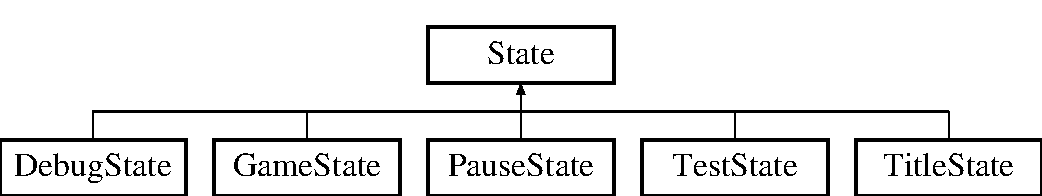
\includegraphics[height=2.000000cm]{classState}
\end{center}
\end{figure}
\subsection*{\-Public \-Member \-Functions}
\begin{DoxyCompactItemize}
\item 
\hypertarget{classState_afede488ff3c1b264bbd07f8aeead84a7_afede488ff3c1b264bbd07f8aeead84a7}{{\bfseries \-State} (\hyperlink{classStateStack}{\-State\-Stack} \&stack, \hyperlink{classContext}{\-Context} context)}\label{classState_afede488ff3c1b264bbd07f8aeead84a7_afede488ff3c1b264bbd07f8aeead84a7}

\item 
\hypertarget{classState_ae261605bc40b7e3959ce5df5457e4942_ae261605bc40b7e3959ce5df5457e4942}{virtual void {\bfseries draw} ()=0}\label{classState_ae261605bc40b7e3959ce5df5457e4942_ae261605bc40b7e3959ce5df5457e4942}

\item 
virtual bool \hyperlink{classState_acd5926bc7a373edff9e57f3ffe94ca13_acd5926bc7a373edff9e57f3ffe94ca13}{update} (sf\-::\-Time dt)=0
\item 
virtual bool \hyperlink{classState_a19965f83460b248c42952aac8d001206_a19965f83460b248c42952aac8d001206}{handle\-Event} (const sf\-::\-Event \&event)=0
\end{DoxyCompactItemize}
\subsection*{\-Protected \-Member \-Functions}
\begin{DoxyCompactItemize}
\item 
\hypertarget{classState_a6763de833ceb9c23df45aff163a4a1cd_a6763de833ceb9c23df45aff163a4a1cd}{void {\bfseries request\-Stack\-Push} (\-States\-::\-I\-D state\-I\-D)}\label{classState_a6763de833ceb9c23df45aff163a4a1cd_a6763de833ceb9c23df45aff163a4a1cd}

\item 
\hypertarget{classState_aa418660892d6161772c907bd8d70f910_aa418660892d6161772c907bd8d70f910}{void {\bfseries request\-Stack\-Pop} ()}\label{classState_aa418660892d6161772c907bd8d70f910_aa418660892d6161772c907bd8d70f910}

\item 
\hypertarget{classState_a4b602bed9bf0179ee5f6748fce340ae6_a4b602bed9bf0179ee5f6748fce340ae6}{void {\bfseries request\-State\-Clear} ()}\label{classState_a4b602bed9bf0179ee5f6748fce340ae6_a4b602bed9bf0179ee5f6748fce340ae6}

\item 
\hypertarget{classState_aec041e226f59f134902ca8671c02788c_aec041e226f59f134902ca8671c02788c}{\hyperlink{classContext}{\-Context} {\bfseries get\-Context} () const }\label{classState_aec041e226f59f134902ca8671c02788c_aec041e226f59f134902ca8671c02788c}

\end{DoxyCompactItemize}
\subsection*{\-Private \-Attributes}
\begin{DoxyCompactItemize}
\item 
\hypertarget{classState_ab7ae9bb2e54a4325acb013c1a51b7b0c_ab7ae9bb2e54a4325acb013c1a51b7b0c}{\hyperlink{classStateStack}{\-State\-Stack} \& {\bfseries m\-Stack}}\label{classState_ab7ae9bb2e54a4325acb013c1a51b7b0c_ab7ae9bb2e54a4325acb013c1a51b7b0c}

\item 
\hypertarget{classState_a7a3d9f2d67529dd7c2eaae143447511b_a7a3d9f2d67529dd7c2eaae143447511b}{\hyperlink{classContext}{\-Context} {\bfseries m\-Context}}\label{classState_a7a3d9f2d67529dd7c2eaae143447511b_a7a3d9f2d67529dd7c2eaae143447511b}

\end{DoxyCompactItemize}


\subsection{\-Detailed \-Description}
\-Represent a state of the application. 

\subsection{\-Member \-Function \-Documentation}
\hypertarget{classState_a19965f83460b248c42952aac8d001206_a19965f83460b248c42952aac8d001206}{\index{\-State@{\-State}!handle\-Event@{handle\-Event}}
\index{handle\-Event@{handle\-Event}!State@{\-State}}
\subsubsection[{handle\-Event}]{\setlength{\rightskip}{0pt plus 5cm}virtual bool {\bf \-State\-::handle\-Event} (
\begin{DoxyParamCaption}
\item[{const sf\-::\-Event \&}]{event}
\end{DoxyParamCaption}
)\hspace{0.3cm}{\ttfamily  \mbox{[}pure virtual\mbox{]}}}}\label{classState_a19965f83460b248c42952aac8d001206_a19965f83460b248c42952aac8d001206}
\-Return false to stop states updating 

\-Implemented in \hyperlink{classPauseState_a685dda66dca3e1c41f4cb02da93c5a8d_a685dda66dca3e1c41f4cb02da93c5a8d}{\-Pause\-State}, \hyperlink{classTestState_a4035262de8411c2f8e2d12980cff089b_a4035262de8411c2f8e2d12980cff089b}{\-Test\-State}, \hyperlink{classTitleState_a91c6ab4d741fe7445d88ed603001971a_a91c6ab4d741fe7445d88ed603001971a}{\-Title\-State}, \hyperlink{classGameState_a000dd3306b1cb9faab5a86774a22aa6d_a000dd3306b1cb9faab5a86774a22aa6d}{\-Game\-State}, and \hyperlink{classDebugState_aef82c5d07e51ab4ea7abcade50370ae2_aef82c5d07e51ab4ea7abcade50370ae2}{\-Debug\-State}.

\hypertarget{classState_acd5926bc7a373edff9e57f3ffe94ca13_acd5926bc7a373edff9e57f3ffe94ca13}{\index{\-State@{\-State}!update@{update}}
\index{update@{update}!State@{\-State}}
\subsubsection[{update}]{\setlength{\rightskip}{0pt plus 5cm}virtual bool {\bf \-State\-::update} (
\begin{DoxyParamCaption}
\item[{sf\-::\-Time}]{dt}
\end{DoxyParamCaption}
)\hspace{0.3cm}{\ttfamily  \mbox{[}pure virtual\mbox{]}}}}\label{classState_acd5926bc7a373edff9e57f3ffe94ca13_acd5926bc7a373edff9e57f3ffe94ca13}
\-Return false to stop states updating 

\-Implemented in \hyperlink{classPauseState_a9d6e9c6d96e140487badbe1da2738fa3_a9d6e9c6d96e140487badbe1da2738fa3}{\-Pause\-State}, \hyperlink{classTestState_affddb89d007d492d4317dbfd1a920b96_affddb89d007d492d4317dbfd1a920b96}{\-Test\-State}, \hyperlink{classGameState_a4ac988f0da5c33b43ff356890fcf9c1c_a4ac988f0da5c33b43ff356890fcf9c1c}{\-Game\-State}, \hyperlink{classDebugState_a6f49614c9b947cedcad131c28e24f885_a6f49614c9b947cedcad131c28e24f885}{\-Debug\-State}, and \hyperlink{classTitleState_aa282ac0c6e22267cb6a7054973d75fdf_aa282ac0c6e22267cb6a7054973d75fdf}{\-Title\-State}.



\-The documentation for this class was generated from the following files\-:\begin{DoxyCompactItemize}
\item 
core/state/\-State.\-hpp\item 
core/state/\-State.\-cpp\end{DoxyCompactItemize}

\hypertarget{classStateStack}{\section{\-State\-Stack \-Class \-Reference}
\label{classStateStack}\index{\-State\-Stack@{\-State\-Stack}}
}


{\ttfamily \#include $<$\-State\-Stack.\-hpp$>$}

\subsection*{\-Classes}
\begin{DoxyCompactItemize}
\item 
struct \hyperlink{structStateStack_1_1PendingChange}{\-Pending\-Change}
\end{DoxyCompactItemize}
\subsection*{\-Public \-Types}
\begin{DoxyCompactItemize}
\item 
enum {\bfseries \-Action} \{ {\bfseries \-Push}, 
{\bfseries \-Pop}, 
{\bfseries \-Clear}
 \}
\end{DoxyCompactItemize}
\subsection*{\-Public \-Member \-Functions}
\begin{DoxyCompactItemize}
\item 
\hypertarget{classStateStack_a237f619f1ee404b3d966fd5dbba98f5a_a237f619f1ee404b3d966fd5dbba98f5a}{{\bfseries \-State\-Stack} (\hyperlink{classAbstractStateFactory}{\-Abstract\-State\-Factory} \&factory, \hyperlink{classContext}{\-Context} context)}\label{classStateStack_a237f619f1ee404b3d966fd5dbba98f5a_a237f619f1ee404b3d966fd5dbba98f5a}

\item 
void \hyperlink{classStateStack_ae90af9f56ce7774d47d0407e2680c27d_ae90af9f56ce7774d47d0407e2680c27d}{update} (sf\-::\-Time dt)
\item 
void \hyperlink{classStateStack_a70d3ffad9da499b8356789115f3e2acf_a70d3ffad9da499b8356789115f3e2acf}{handle\-Event} (const sf\-::\-Event \&event)
\item 
void \hyperlink{classStateStack_a0990b973b2a0bdf8fad2f326e564931a_a0990b973b2a0bdf8fad2f326e564931a}{draw} ()
\item 
void \hyperlink{classStateStack_a5d4d9c5e5d95be4392ef2c95fdc0c047_a5d4d9c5e5d95be4392ef2c95fdc0c047}{push\-State} (\-States\-::\-I\-D id)
\item 
\hypertarget{classStateStack_a7e050a57b798295c2344f1318765b5ee_a7e050a57b798295c2344f1318765b5ee}{void {\bfseries pop\-State} ()}\label{classStateStack_a7e050a57b798295c2344f1318765b5ee_a7e050a57b798295c2344f1318765b5ee}

\item 
\hypertarget{classStateStack_a49f0703d4037c3bf63494e64cb09898d_a49f0703d4037c3bf63494e64cb09898d}{void {\bfseries clear\-States} ()}\label{classStateStack_a49f0703d4037c3bf63494e64cb09898d_a49f0703d4037c3bf63494e64cb09898d}

\item 
\hypertarget{classStateStack_a63a73898d24eb0a68cac0215a9fda4fc_a63a73898d24eb0a68cac0215a9fda4fc}{bool {\bfseries is\-Empty} () const }\label{classStateStack_a63a73898d24eb0a68cac0215a9fda4fc_a63a73898d24eb0a68cac0215a9fda4fc}

\end{DoxyCompactItemize}
\subsection*{\-Private \-Types}
\begin{DoxyCompactItemize}
\item 
\hypertarget{classStateStack_a98d8e25ed9ad5889b145982b8a167cf0_a98d8e25ed9ad5889b145982b8a167cf0}{typedef std\-::vector$<$ \hyperlink{classState}{\-State} $\ast$ $>$ {\bfseries \-State\-Ptr\-Vector}}\label{classStateStack_a98d8e25ed9ad5889b145982b8a167cf0_a98d8e25ed9ad5889b145982b8a167cf0}

\item 
\hypertarget{classStateStack_aa3a35524fb99f5d12b4276bdf2a56744_aa3a35524fb99f5d12b4276bdf2a56744}{typedef std\-::vector\*
$<$ \hyperlink{structStateStack_1_1PendingChange}{\-Pending\-Change} $>$ {\bfseries \-Pending\-Change\-Vector}}\label{classStateStack_aa3a35524fb99f5d12b4276bdf2a56744_aa3a35524fb99f5d12b4276bdf2a56744}

\end{DoxyCompactItemize}
\subsection*{\-Private \-Member \-Functions}
\begin{DoxyCompactItemize}
\item 
\hypertarget{classStateStack_af664f95954b4621175c9fc0f9d30fdf0_af664f95954b4621175c9fc0f9d30fdf0}{void {\bfseries apply\-Pending\-Changes} ()}\label{classStateStack_af664f95954b4621175c9fc0f9d30fdf0_af664f95954b4621175c9fc0f9d30fdf0}

\end{DoxyCompactItemize}
\subsection*{\-Private \-Attributes}
\begin{DoxyCompactItemize}
\item 
\hypertarget{classStateStack_a1e91ad8bee74b8d3b0a79516334f876e_a1e91ad8bee74b8d3b0a79516334f876e}{\-State\-Ptr\-Vector {\bfseries m\-Stack}}\label{classStateStack_a1e91ad8bee74b8d3b0a79516334f876e_a1e91ad8bee74b8d3b0a79516334f876e}

\item 
\hypertarget{classStateStack_adbc8d0b3e30caf552c705ee189a5bcbb_adbc8d0b3e30caf552c705ee189a5bcbb}{\-Pending\-Change\-Vector {\bfseries m\-Pending\-List}}\label{classStateStack_adbc8d0b3e30caf552c705ee189a5bcbb_adbc8d0b3e30caf552c705ee189a5bcbb}

\item 
\hypertarget{classStateStack_ac5e8ff25cd93f9c4a4345be08b6da7ea_ac5e8ff25cd93f9c4a4345be08b6da7ea}{\hyperlink{classContext}{\-Context} {\bfseries m\-Context}}\label{classStateStack_ac5e8ff25cd93f9c4a4345be08b6da7ea_ac5e8ff25cd93f9c4a4345be08b6da7ea}

\item 
\hypertarget{classStateStack_a10fc35b00720872d373ea694a6a911e0_a10fc35b00720872d373ea694a6a911e0}{\hyperlink{classAbstractStateFactory}{\-Abstract\-State\-Factory} \& {\bfseries m\-Factory}}\label{classStateStack_a10fc35b00720872d373ea694a6a911e0_a10fc35b00720872d373ea694a6a911e0}

\end{DoxyCompactItemize}


\subsection{\-Detailed \-Description}
\-Manage states of the application. 

\subsection{\-Member \-Function \-Documentation}
\hypertarget{classStateStack_a0990b973b2a0bdf8fad2f326e564931a_a0990b973b2a0bdf8fad2f326e564931a}{\index{\-State\-Stack@{\-State\-Stack}!draw@{draw}}
\index{draw@{draw}!StateStack@{\-State\-Stack}}
\subsubsection[{draw}]{\setlength{\rightskip}{0pt plus 5cm}void {\bf \-State\-Stack\-::draw} (
\begin{DoxyParamCaption}
{}
\end{DoxyParamCaption}
)}}\label{classStateStack_a0990b973b2a0bdf8fad2f326e564931a_a0990b973b2a0bdf8fad2f326e564931a}
\-Draw all the states from the bottom \hypertarget{classStateStack_a70d3ffad9da499b8356789115f3e2acf_a70d3ffad9da499b8356789115f3e2acf}{\index{\-State\-Stack@{\-State\-Stack}!handle\-Event@{handle\-Event}}
\index{handle\-Event@{handle\-Event}!StateStack@{\-State\-Stack}}
\subsubsection[{handle\-Event}]{\setlength{\rightskip}{0pt plus 5cm}void {\bf \-State\-Stack\-::handle\-Event} (
\begin{DoxyParamCaption}
\item[{const sf\-::\-Event \&}]{event}
\end{DoxyParamCaption}
)}}\label{classStateStack_a70d3ffad9da499b8356789115f3e2acf_a70d3ffad9da499b8356789115f3e2acf}
\-Notify states from the top 
\begin{DoxyParams}{\-Parameters}
{\em event} & \-Event to treat \\
\hline
\end{DoxyParams}
\hypertarget{classStateStack_a5d4d9c5e5d95be4392ef2c95fdc0c047_a5d4d9c5e5d95be4392ef2c95fdc0c047}{\index{\-State\-Stack@{\-State\-Stack}!push\-State@{push\-State}}
\index{push\-State@{push\-State}!StateStack@{\-State\-Stack}}
\subsubsection[{push\-State}]{\setlength{\rightskip}{0pt plus 5cm}void {\bf \-State\-Stack\-::push\-State} (
\begin{DoxyParamCaption}
\item[{\-States\-::\-I\-D}]{id}
\end{DoxyParamCaption}
)}}\label{classStateStack_a5d4d9c5e5d95be4392ef2c95fdc0c047_a5d4d9c5e5d95be4392ef2c95fdc0c047}
\-Set the top active state 
\begin{DoxyParams}{\-Parameters}
{\em id} & \-Id of the state, accordly to the id into the \-State\-Factory \\
\hline
\end{DoxyParams}
\hypertarget{classStateStack_ae90af9f56ce7774d47d0407e2680c27d_ae90af9f56ce7774d47d0407e2680c27d}{\index{\-State\-Stack@{\-State\-Stack}!update@{update}}
\index{update@{update}!StateStack@{\-State\-Stack}}
\subsubsection[{update}]{\setlength{\rightskip}{0pt plus 5cm}void {\bf \-State\-Stack\-::update} (
\begin{DoxyParamCaption}
\item[{sf\-::\-Time}]{dt}
\end{DoxyParamCaption}
)}}\label{classStateStack_ae90af9f56ce7774d47d0407e2680c27d_ae90af9f56ce7774d47d0407e2680c27d}
\-Update all the states 
\begin{DoxyParams}{\-Parameters}
{\em dt} & \-Time elapsed since the latest call \\
\hline
\end{DoxyParams}


\-The documentation for this class was generated from the following files\-:\begin{DoxyCompactItemize}
\item 
core/state/\-State\-Stack.\-hpp\item 
core/state/\-State\-Stack.\-cpp\end{DoxyCompactItemize}

\hypertarget{classTestState}{\section{\-Test\-State \-Class \-Reference}
\label{classTestState}\index{\-Test\-State@{\-Test\-State}}
}
\-Inheritance diagram for \-Test\-State\-:\begin{figure}[H]
\begin{center}
\leavevmode
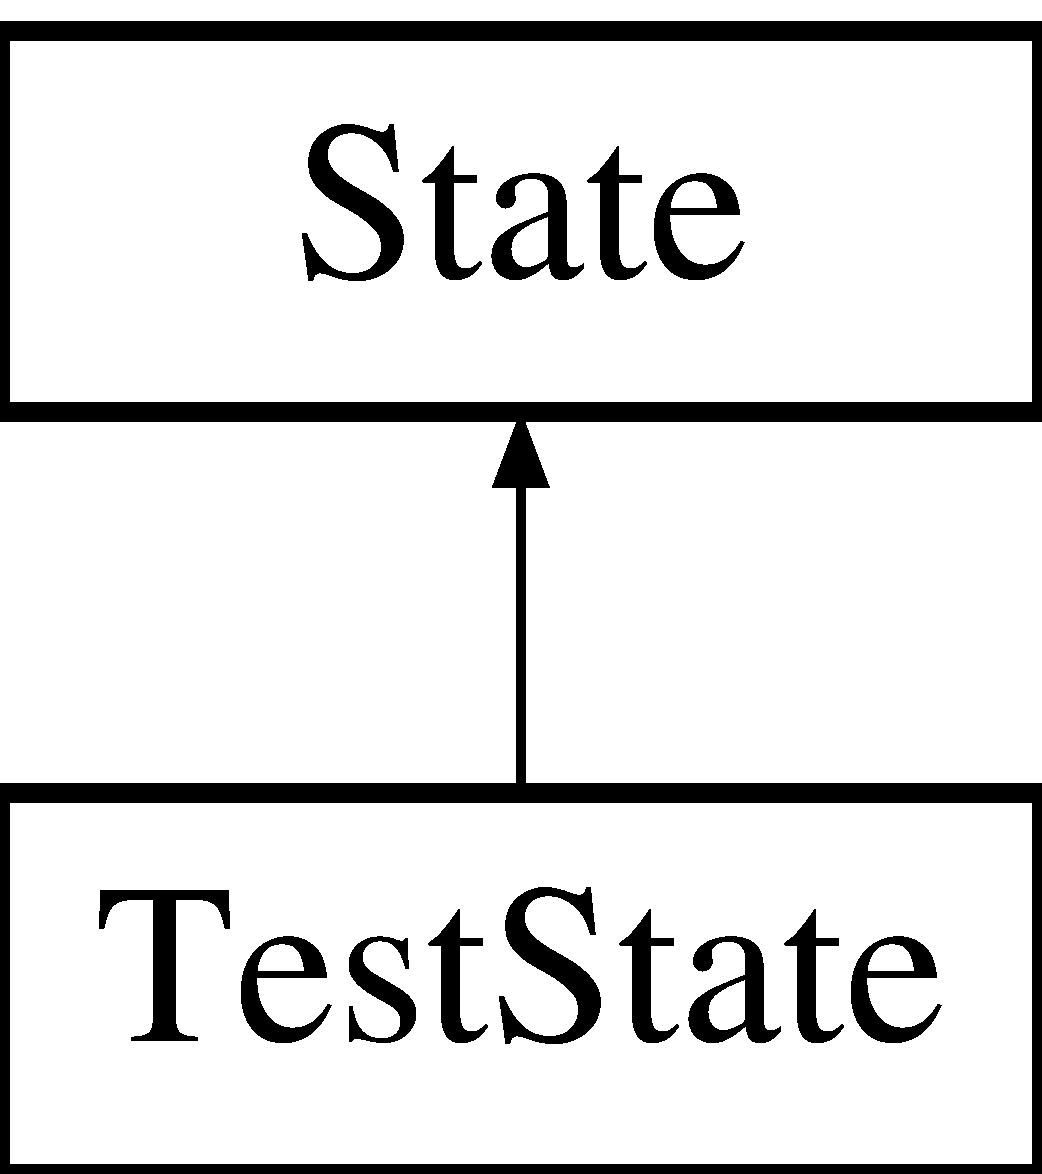
\includegraphics[height=2.000000cm]{classTestState}
\end{center}
\end{figure}
\subsection*{\-Public \-Member \-Functions}
\begin{DoxyCompactItemize}
\item 
\hypertarget{classTestState_a88a30c86aefe8e7631b1fef5b63d2c9a_a88a30c86aefe8e7631b1fef5b63d2c9a}{{\bfseries \-Test\-State} (\hyperlink{classStateStack}{\-State\-Stack} \&stack, \hyperlink{classContext}{\-Context} \&context)}\label{classTestState_a88a30c86aefe8e7631b1fef5b63d2c9a_a88a30c86aefe8e7631b1fef5b63d2c9a}

\item 
virtual bool \hyperlink{classTestState_a4035262de8411c2f8e2d12980cff089b_a4035262de8411c2f8e2d12980cff089b}{handle\-Event} (const sf\-::\-Event \&event)
\item 
virtual bool \hyperlink{classTestState_affddb89d007d492d4317dbfd1a920b96_affddb89d007d492d4317dbfd1a920b96}{update} (sf\-::\-Time dt)
\item 
\hypertarget{classTestState_af4baacd03a87b3a8abbf8e9fe0e989a4_af4baacd03a87b3a8abbf8e9fe0e989a4}{virtual void {\bfseries draw} ()}\label{classTestState_af4baacd03a87b3a8abbf8e9fe0e989a4_af4baacd03a87b3a8abbf8e9fe0e989a4}

\end{DoxyCompactItemize}
\subsection*{\-Private \-Attributes}
\begin{DoxyCompactItemize}
\item 
\hypertarget{classTestState_a58a5123af76eca1d1c90fe2aca4be2d3_a58a5123af76eca1d1c90fe2aca4be2d3}{\hyperlink{classMap}{\-Map} $\ast$ {\bfseries carte}}\label{classTestState_a58a5123af76eca1d1c90fe2aca4be2d3_a58a5123af76eca1d1c90fe2aca4be2d3}

\end{DoxyCompactItemize}


\subsection{\-Member \-Function \-Documentation}
\hypertarget{classTestState_a4035262de8411c2f8e2d12980cff089b_a4035262de8411c2f8e2d12980cff089b}{\index{\-Test\-State@{\-Test\-State}!handle\-Event@{handle\-Event}}
\index{handle\-Event@{handle\-Event}!TestState@{\-Test\-State}}
\subsubsection[{handle\-Event}]{\setlength{\rightskip}{0pt plus 5cm}bool {\bf \-Test\-State\-::handle\-Event} (
\begin{DoxyParamCaption}
\item[{const sf\-::\-Event \&}]{event}
\end{DoxyParamCaption}
)\hspace{0.3cm}{\ttfamily  \mbox{[}virtual\mbox{]}}}}\label{classTestState_a4035262de8411c2f8e2d12980cff089b_a4035262de8411c2f8e2d12980cff089b}
\-Return false to stop states updating 

\-Implements \hyperlink{classState_a19965f83460b248c42952aac8d001206_a19965f83460b248c42952aac8d001206}{\-State}.

\hypertarget{classTestState_affddb89d007d492d4317dbfd1a920b96_affddb89d007d492d4317dbfd1a920b96}{\index{\-Test\-State@{\-Test\-State}!update@{update}}
\index{update@{update}!TestState@{\-Test\-State}}
\subsubsection[{update}]{\setlength{\rightskip}{0pt plus 5cm}bool {\bf \-Test\-State\-::update} (
\begin{DoxyParamCaption}
\item[{sf\-::\-Time}]{dt}
\end{DoxyParamCaption}
)\hspace{0.3cm}{\ttfamily  \mbox{[}virtual\mbox{]}}}}\label{classTestState_affddb89d007d492d4317dbfd1a920b96_affddb89d007d492d4317dbfd1a920b96}
\-Return false to stop states updating 

\-Implements \hyperlink{classState_acd5926bc7a373edff9e57f3ffe94ca13_acd5926bc7a373edff9e57f3ffe94ca13}{\-State}.



\-The documentation for this class was generated from the following files\-:\begin{DoxyCompactItemize}
\item 
gameplay/\-Test\-State.\-hpp\item 
gameplay/\-Test\-State.\-cpp\end{DoxyCompactItemize}

\hypertarget{classTextureHolder}{\section{\-Texture\-Holder \-Class \-Reference}
\label{classTextureHolder}\index{\-Texture\-Holder@{\-Texture\-Holder}}
}


{\ttfamily \#include $<$\-Texture\-Holder.\-hpp$>$}

\subsection*{\-Public \-Member \-Functions}
\begin{DoxyCompactItemize}
\item 
\hypertarget{classTextureHolder_a7a88fb0da3c2754e80026d65eb024551_a7a88fb0da3c2754e80026d65eb024551}{void {\bfseries load} (\-Textures\-::\-I\-D id, const std\-::string \&filename)}\label{classTextureHolder_a7a88fb0da3c2754e80026d65eb024551_a7a88fb0da3c2754e80026d65eb024551}

\item 
\hypertarget{classTextureHolder_a3a319ddaa24fb4e990af3d5c6b58ff4d_a3a319ddaa24fb4e990af3d5c6b58ff4d}{sf\-::\-Texture \& {\bfseries get} (\-Textures\-::\-I\-D id)}\label{classTextureHolder_a3a319ddaa24fb4e990af3d5c6b58ff4d_a3a319ddaa24fb4e990af3d5c6b58ff4d}

\item 
\hypertarget{classTextureHolder_af1f14ad2ea40a6868a04e874105ce4a2_af1f14ad2ea40a6868a04e874105ce4a2}{const sf\-::\-Texture \& {\bfseries get} (\-Textures\-::\-I\-D id) const }\label{classTextureHolder_af1f14ad2ea40a6868a04e874105ce4a2_af1f14ad2ea40a6868a04e874105ce4a2}

\end{DoxyCompactItemize}
\subsection*{\-Private \-Types}
\begin{DoxyCompactItemize}
\item 
\hypertarget{classTextureHolder_a0413de5ea86e66ff2c9e3b48273b59a9_a0413de5ea86e66ff2c9e3b48273b59a9}{typedef std\-::map$<$ \-Textures\-::\-I\-D, \*
sf\-::\-Texture $\ast$ $>$ {\bfseries \-Texture\-Map}}\label{classTextureHolder_a0413de5ea86e66ff2c9e3b48273b59a9_a0413de5ea86e66ff2c9e3b48273b59a9}

\end{DoxyCompactItemize}
\subsection*{\-Private \-Attributes}
\begin{DoxyCompactItemize}
\item 
\hypertarget{classTextureHolder_a8f7a9a3896c84ab877f0c5272daf708a_a8f7a9a3896c84ab877f0c5272daf708a}{\-Texture\-Map {\bfseries m\-Texture\-Map}}\label{classTextureHolder_a8f7a9a3896c84ab877f0c5272daf708a_a8f7a9a3896c84ab877f0c5272daf708a}

\item 
\hypertarget{classTextureHolder_a31d4a58279fde9b88a6b2db1dca80b2d_a31d4a58279fde9b88a6b2db1dca80b2d}{sf\-::\-Texture {\bfseries m\-Default\-Texture}}\label{classTextureHolder_a31d4a58279fde9b88a6b2db1dca80b2d_a31d4a58279fde9b88a6b2db1dca80b2d}

\end{DoxyCompactItemize}


\subsection{\-Detailed \-Description}
\-Manage textures. \-Avoid double resource. 

\-The documentation for this class was generated from the following files\-:\begin{DoxyCompactItemize}
\item 
core/\-Texture\-Holder.\-hpp\item 
core/\-Texture\-Holder.\-cpp\end{DoxyCompactItemize}

\hypertarget{classTitleState}{\section{\-Title\-State \-Class \-Reference}
\label{classTitleState}\index{\-Title\-State@{\-Title\-State}}
}
\-Inheritance diagram for \-Title\-State\-:\begin{figure}[H]
\begin{center}
\leavevmode
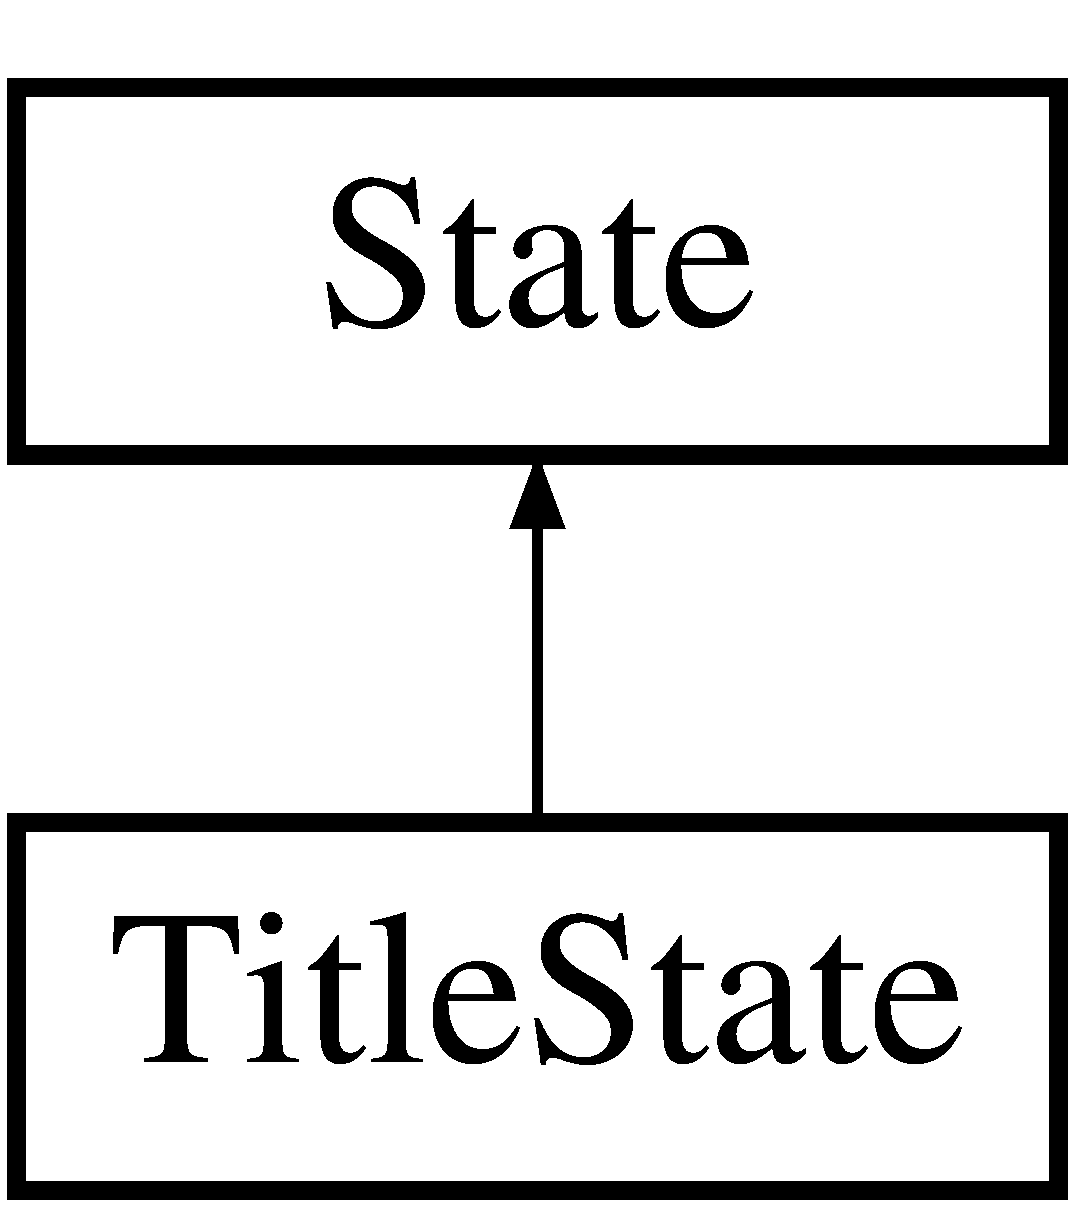
\includegraphics[height=2.000000cm]{classTitleState}
\end{center}
\end{figure}
\subsection*{\-Public \-Member \-Functions}
\begin{DoxyCompactItemize}
\item 
\hypertarget{classTitleState_a7e8f520cb4fc6d0640aa79bc068bab86_a7e8f520cb4fc6d0640aa79bc068bab86}{{\bfseries \-Title\-State} (\hyperlink{classStateStack}{\-State\-Stack} \&stack, \hyperlink{classContext}{\-Context} \&context)}\label{classTitleState_a7e8f520cb4fc6d0640aa79bc068bab86_a7e8f520cb4fc6d0640aa79bc068bab86}

\item 
\hypertarget{classTitleState_ae12beafe5aad6929a56089942de1220e_ae12beafe5aad6929a56089942de1220e}{virtual void {\bfseries draw} ()}\label{classTitleState_ae12beafe5aad6929a56089942de1220e_ae12beafe5aad6929a56089942de1220e}

\item 
virtual bool \hyperlink{classTitleState_aa282ac0c6e22267cb6a7054973d75fdf_aa282ac0c6e22267cb6a7054973d75fdf}{update} (sf\-::\-Time dt)
\item 
virtual bool \hyperlink{classTitleState_a91c6ab4d741fe7445d88ed603001971a_a91c6ab4d741fe7445d88ed603001971a}{handle\-Event} (const sf\-::\-Event \&event)
\end{DoxyCompactItemize}


\subsection{\-Member \-Function \-Documentation}
\hypertarget{classTitleState_a91c6ab4d741fe7445d88ed603001971a_a91c6ab4d741fe7445d88ed603001971a}{\index{\-Title\-State@{\-Title\-State}!handle\-Event@{handle\-Event}}
\index{handle\-Event@{handle\-Event}!TitleState@{\-Title\-State}}
\subsubsection[{handle\-Event}]{\setlength{\rightskip}{0pt plus 5cm}bool {\bf \-Title\-State\-::handle\-Event} (
\begin{DoxyParamCaption}
\item[{const sf\-::\-Event \&}]{event}
\end{DoxyParamCaption}
)\hspace{0.3cm}{\ttfamily  \mbox{[}virtual\mbox{]}}}}\label{classTitleState_a91c6ab4d741fe7445d88ed603001971a_a91c6ab4d741fe7445d88ed603001971a}
\-Return false to stop states updating 

\-Implements \hyperlink{classState_a19965f83460b248c42952aac8d001206_a19965f83460b248c42952aac8d001206}{\-State}.

\hypertarget{classTitleState_aa282ac0c6e22267cb6a7054973d75fdf_aa282ac0c6e22267cb6a7054973d75fdf}{\index{\-Title\-State@{\-Title\-State}!update@{update}}
\index{update@{update}!TitleState@{\-Title\-State}}
\subsubsection[{update}]{\setlength{\rightskip}{0pt plus 5cm}bool {\bf \-Title\-State\-::update} (
\begin{DoxyParamCaption}
\item[{sf\-::\-Time}]{dt}
\end{DoxyParamCaption}
)\hspace{0.3cm}{\ttfamily  \mbox{[}virtual\mbox{]}}}}\label{classTitleState_aa282ac0c6e22267cb6a7054973d75fdf_aa282ac0c6e22267cb6a7054973d75fdf}
\-Return false to stop states updating 

\-Implements \hyperlink{classState_acd5926bc7a373edff9e57f3ffe94ca13_acd5926bc7a373edff9e57f3ffe94ca13}{\-State}.



\-The documentation for this class was generated from the following files\-:\begin{DoxyCompactItemize}
\item 
gameplay/\-Title\-State.\-hpp\item 
gameplay/\-Title\-State.\-cpp\end{DoxyCompactItemize}

\printindex
\end{document}
